\hyt{pohadka}
\song{Pohádka}

\intro{
	
\vspace{-25pt}
\hspace{20pt}
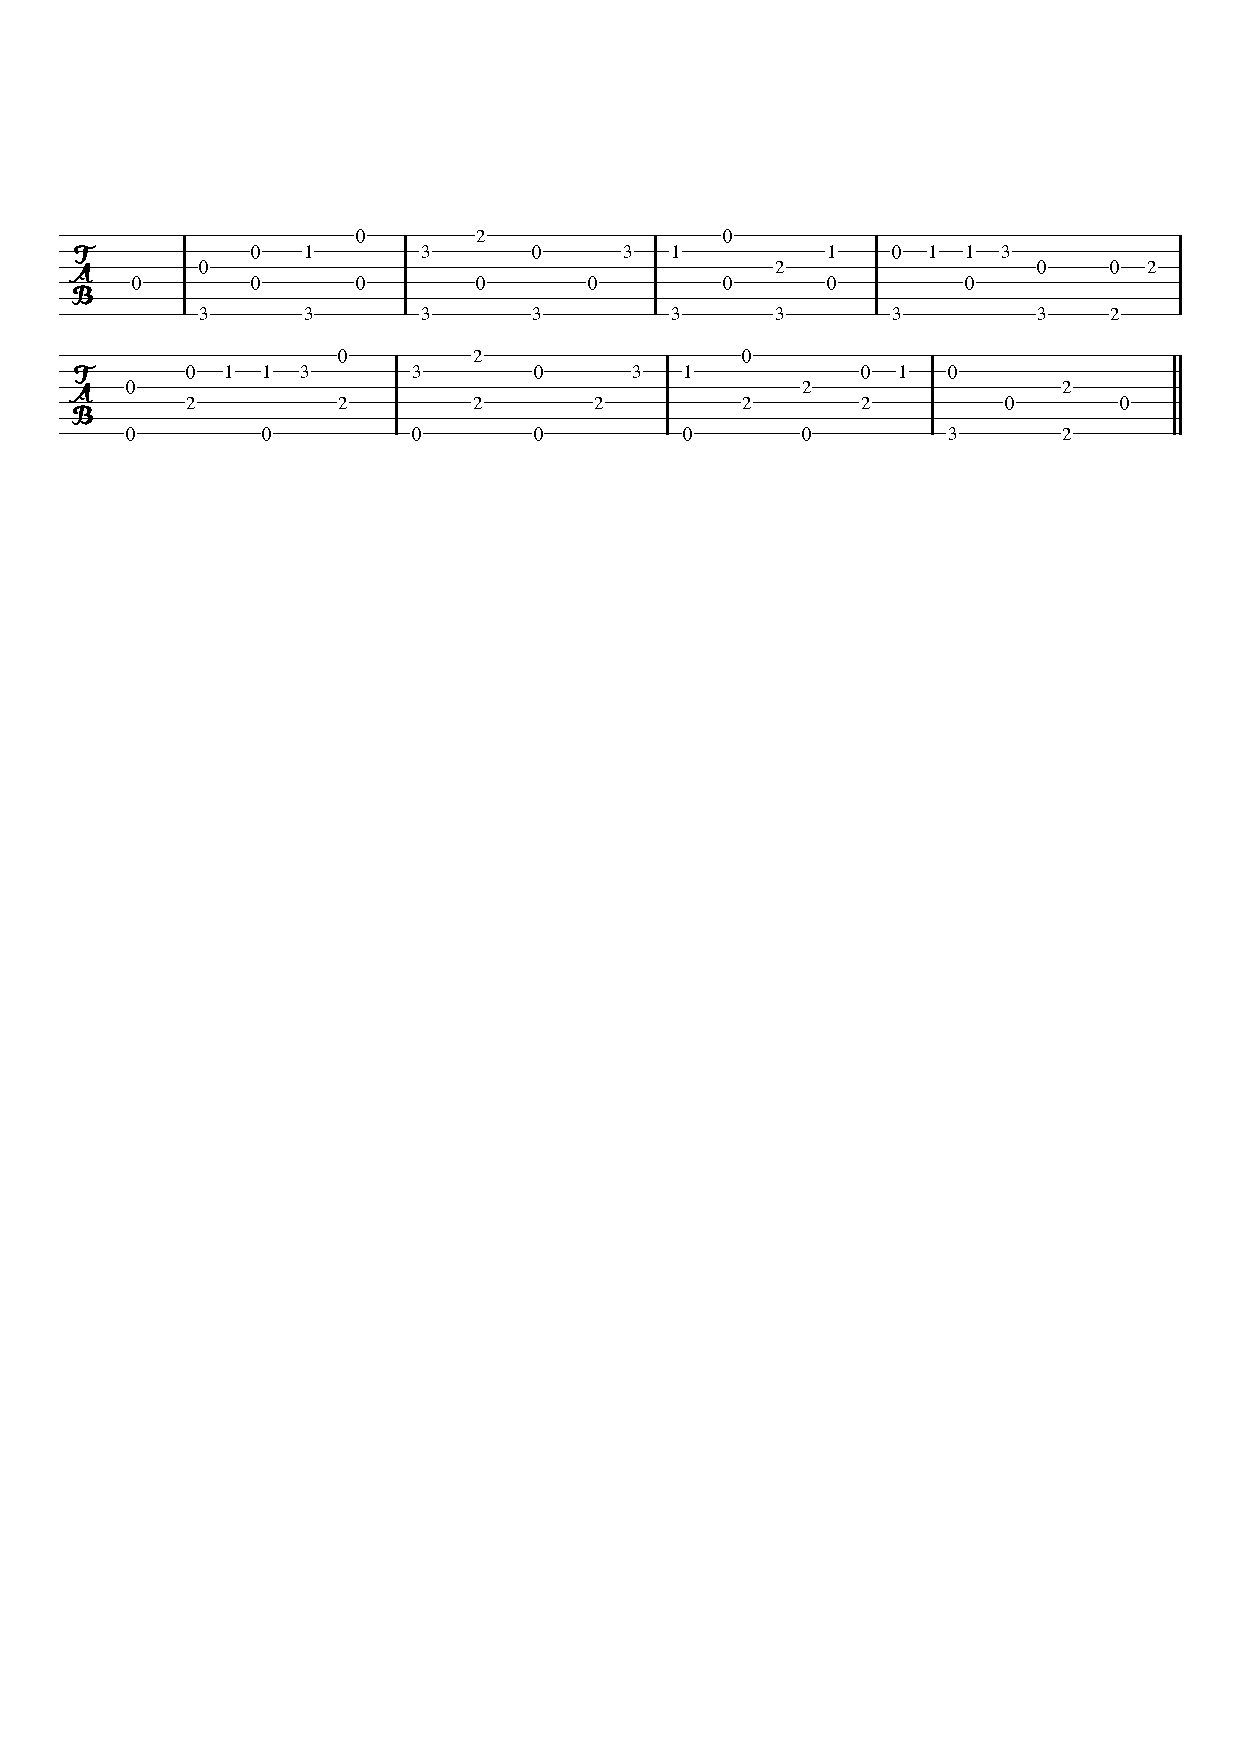
\includegraphics[width=\linewidth]{scores/pohadka.pdf}
}

\vspace{10pt}
\rec{
Takhle nějak to bylo: Jedlo se, zpívalo, pilo,\\
princezna zářila štěstím v hotelu nad náměstím.\\
\vinv
Drak hlídal u dveří sálu, na krku pletenou šálu,\\
dědové Vševědi okolo Popelky žvatlavě slibují šaty a kabelky.\\
\vinv
Každý si odnáší kousíček úsměvu, dešťový mraky se chystaly ke zpěvu,\\
hosté se sjíždějí k veliké veselce, paprsky luceren metají kozelce.\\
\vinv
A stíny ořechů orvaných dohola pletou se letícím kočárům pod kola.\\
Šmudla si přivezl v odřeným Wartburgu kámošku z dětství, prej nějakou Sněhurku.\\
\vinv
Vrátný se zohýbá pro tučné spropitné, a kdo mu proklouzne, tak toho nechytne.\\
Kouzelník za dvacku vykouzlí pět bonů a vítr na věži opřel se do zvonů.\\
\vinv
Honzové, princové, víly i sudičky chopí se poháru, nože i vidličky.\\
\uv{Na zdraví nevěsty, na zdraví ženicha!}, dvě sousta do kapsy a jedno do břicha.\\
\vinv
Náhle se za oknem objevil skřítek, rozhrnul oponu z máminých kytek,\\
pěkně se usmál a pěkně se podíval, a pak mi potichu do ucha zazpíval.
}
\vspace{-15pt}

\refrain{
\chord{G}Dej mi ruku \chord{D}svou, studenou \chord{Em}od okenních \chord{Hm}skel,\\
všichni tě \chord{C}mezi sebe \chord{Hm}zvou a \chord{C}já jsem \chord{D}tu proto, \chord{G}abys šel.

\vspace{0pt}
\hspace{20pt}
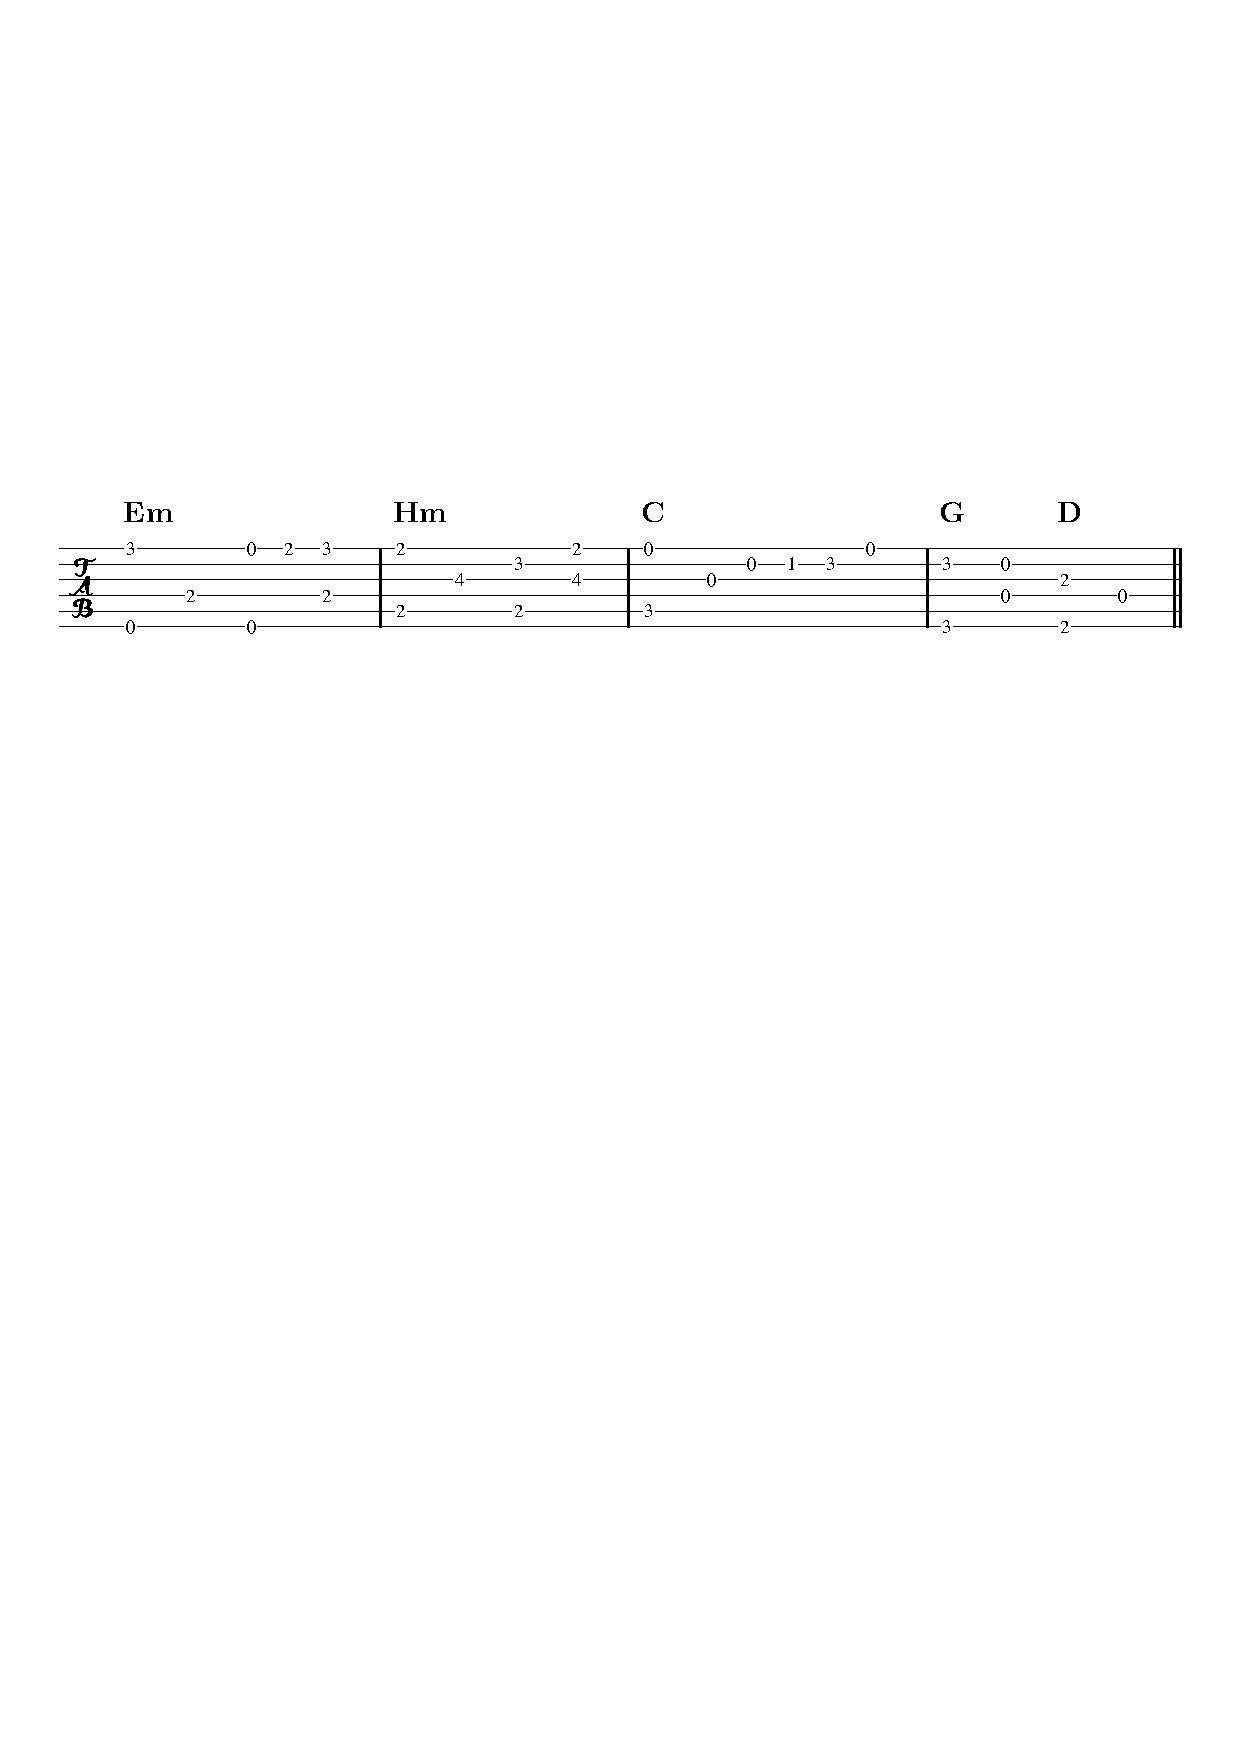
\includegraphics[width=\linewidth]{scores/pohadkaref.pdf}
}

\rec{
Na plný obrátky letíme světem, všechny ty pohádky patřily dětem.\\
Píšeš mi z ciziny zoufalý dopisy, koukám se z okna a vzpomínám na kdysi,\\
\vinv
jak se mi za oknem objevil skřítek, rozhrnul oponu z máminých kytek.\\
Pěkně se usmál a pěkně se podíval, a pak mi potichu do ucha zazpíval.
} \refsm{} $\times 2$
\newpage
